% !TeX root = ../../main.tex

\section{Zbiory danych}

Do przeprowadzenia eksperymentów użyto dwóch zbiorów danych, pozyskanych od firmy ``BLUE''. Jeden zbiór, zwany dalej zbiorem \textit{high} pochodzi z kamer ustawianych ponad kortem. Drugi zbiór, zwany dalej zbiorem \textit{low}, pochodzi z kamer sytuowanych na podłodze, tuż przy liniach kortu.

\begin{figure}[!htb]
  \minipage{0.45\textwidth}
    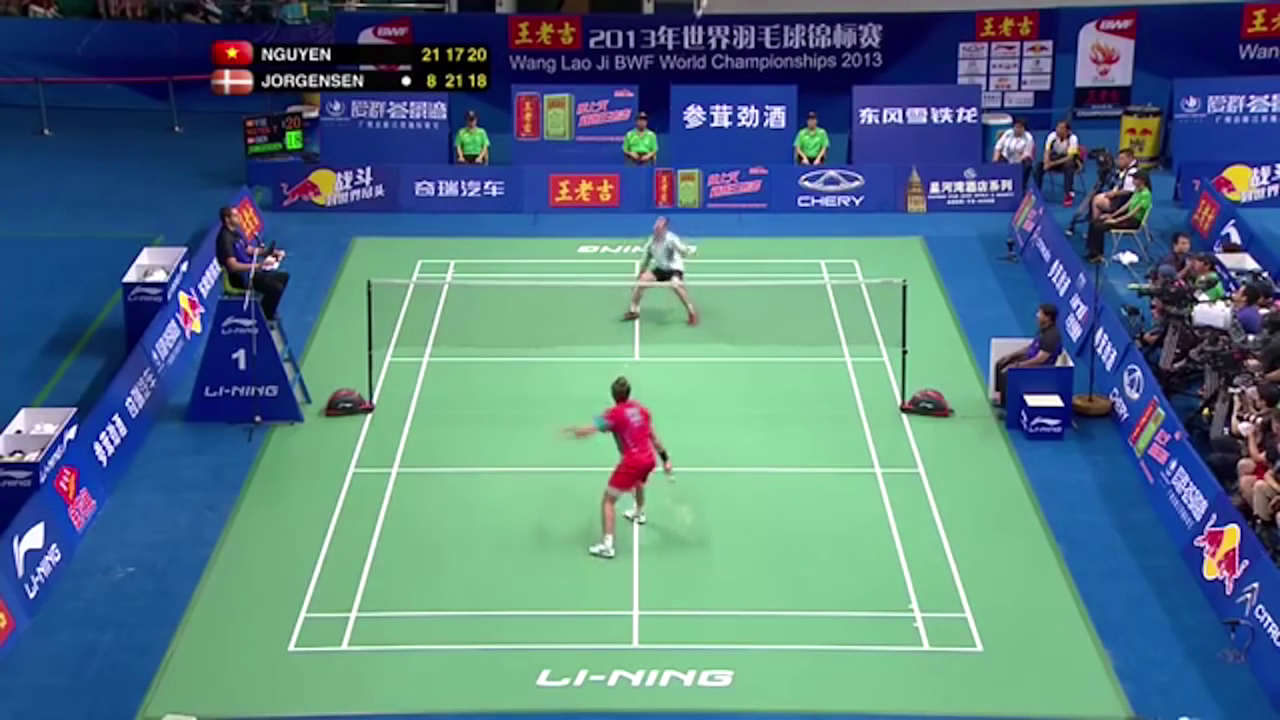
\includegraphics[width=\linewidth]{../badminton/datasets/badminton_high/train/test_court2-00002.png}
    \caption{Przykładowy obraz ze zbioru danych \textit{high}}
  \endminipage\hfill
  \minipage{0.45\textwidth}
    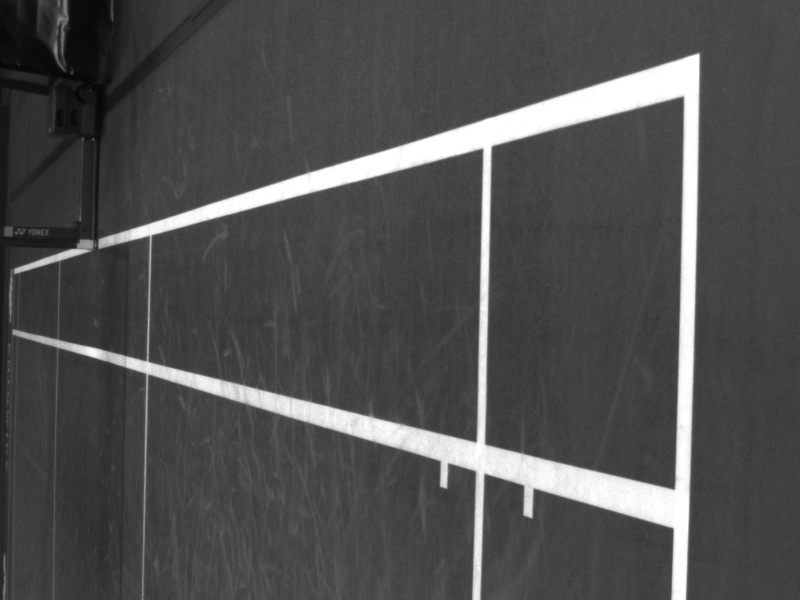
\includegraphics[width=\linewidth]{../badminton/datasets/badminton_low/train/1564909032792410075.jpg}
    \caption{Przykładowy obraz ze zbioru danych \textit{low}}
  \endminipage\hfill
  \end{figure}
